% This is samplepaper.tex, a sample chapter demonstrating the
% LLNCS macro package for Springer Computer Science proceedings;
% Version 2.21 of 2022/01/12
%
\documentclass[runningheads]{llncs}
%
\usepackage[T1]{fontenc}
% T1 fonts will be used to generate the final print and online PDFs,
% so please use T1 fonts in your manuscript whenever possible.
% Other font encondings may result in incorrect characters.
%
\usepackage{graphicx}
\usepackage{booktabs}
\usepackage{tabularx}
\usepackage{adjustbox}
\usepackage{graphicx}
\usepackage{subcaption}
\usepackage{array} 
\usepackage{float}
\usepackage{multirow}
\usepackage{subcaption}
\usepackage{tabularx} % 在导言区添加此宏包
\usepackage{booktabs}  % 专业表格线
\usepackage{array}     % 提供更好的列格式控制

\usepackage{caption}
\captionsetup{
    labelfont=bf,    % 加粗标签
    labelsep=period, % 强制使用句点(.)而不是冒号(:)
}

\newcolumntype{C}{>{\centering\arraybackslash}X} % 定义居中列类型
\usepackage{cleveref}
\crefformat{figure}{\textbf{Fig.~#2#1#3}}



%\newcolumntype{C}{>{\centering\arraybackslash}X} % 定义居中列类型
% Used for displaying a sample figure. If possible, figure files should
% be included in EPS format.
%
% If you use the hyperref package, please uncomment the following two lines
% to display URLs in blue roman font according to Springer's eBook style:
%\usepackage{color}
%\renewcommand\UrlFont{\color{blue}\rmfamily}

\begin{document}

\title{Real-world Feasibility Analysis of ACT Algorithm for Robotic Manipulation on Home}

%\titlerunning{Abbreviated paper title}
% If the paper title is too long for the running head, you can set
% an abbreviated paper title here
\titlerunning{Real-world Feasibility Analysis of ACT Algorithm for Robotic Manipulation}  % 页眉显示的短标题
\author{
  Junlin Huang\inst{1} \and
  Feihong Liu\inst{1} \and
  Siyu Wang\inst{1} \and
  Yang Yang\inst{1} \and
  Yuhang Li\inst{1} \and
  Qiuyue Che\inst{1} \and
  Qiushuang Liu\inst{1} \and
  Deping Li\inst{1}\thanks{Corresponding author: lideping@jnu.edu.cn}
}

\authorrunning{Huang et al.}  % 保持运行标题简洁


\institute{
  School of Intelligent Systems Science and Engineering/JNU-Industry School of Artificial Intelligence,   % 补充学院名称
  Jinan University, 
  Zhuhai 519070, China \\ % 补充邮编
  \email{lideping@jnu.edu.cn}  % 明确标记通讯作者邮箱
  %\email{gzhuangjunlin@163.com}  
}


\maketitle




%
\begin{abstract}
Imitation learning allows robots to efficiently acquire complex tasks that are challenging to program manually. By learning from demonstrations, robots can adapt to new environments and task variations while enabling intuitive human-robot interaction. However, hardware constraints—such as motion limitations and sensory precision—often reduce its effectiveness. To mitigate these issues, we evaluate the Action Chunking with Transformers (ACT) algorithm, which reduces compounding errors and enhances learning efficiency. Through systematic experiments across two distinct task objectives under varying conditions, we assess ACT’s real-world applicability and its potential to accelerate robotic deployment.


\keywords{Imitation Learning  \and Behavioral Cloning (BC) \and Action Chunking with Transformers (ACT).}
\end{abstract}
%
%
%
\section{Introduction}
The ACT algorithm creates low-cost imitation learning by combining action chunking and temporal ensemble to address error accumulation in behavioral cloning. It trains neural networks on state-action data, significantly reducing time-amplified execution errors in industrial precision tasks. 
 
 As shown in Fig.~\ref{fig1}(a), the algorithm employs action chunking and temporal ensemble techniques during training. With a fixed chunk size k, the agent receives environmental observations every k steps and executes k sequential actions. This design effectively reduces historical error accumulation. To ensure motion continuity, the algorithm queries the policy at every timestep, generating overlapping predicted actions that are then smoothly blended through temporal ensemble using exponential weighting.

\begin{figure}
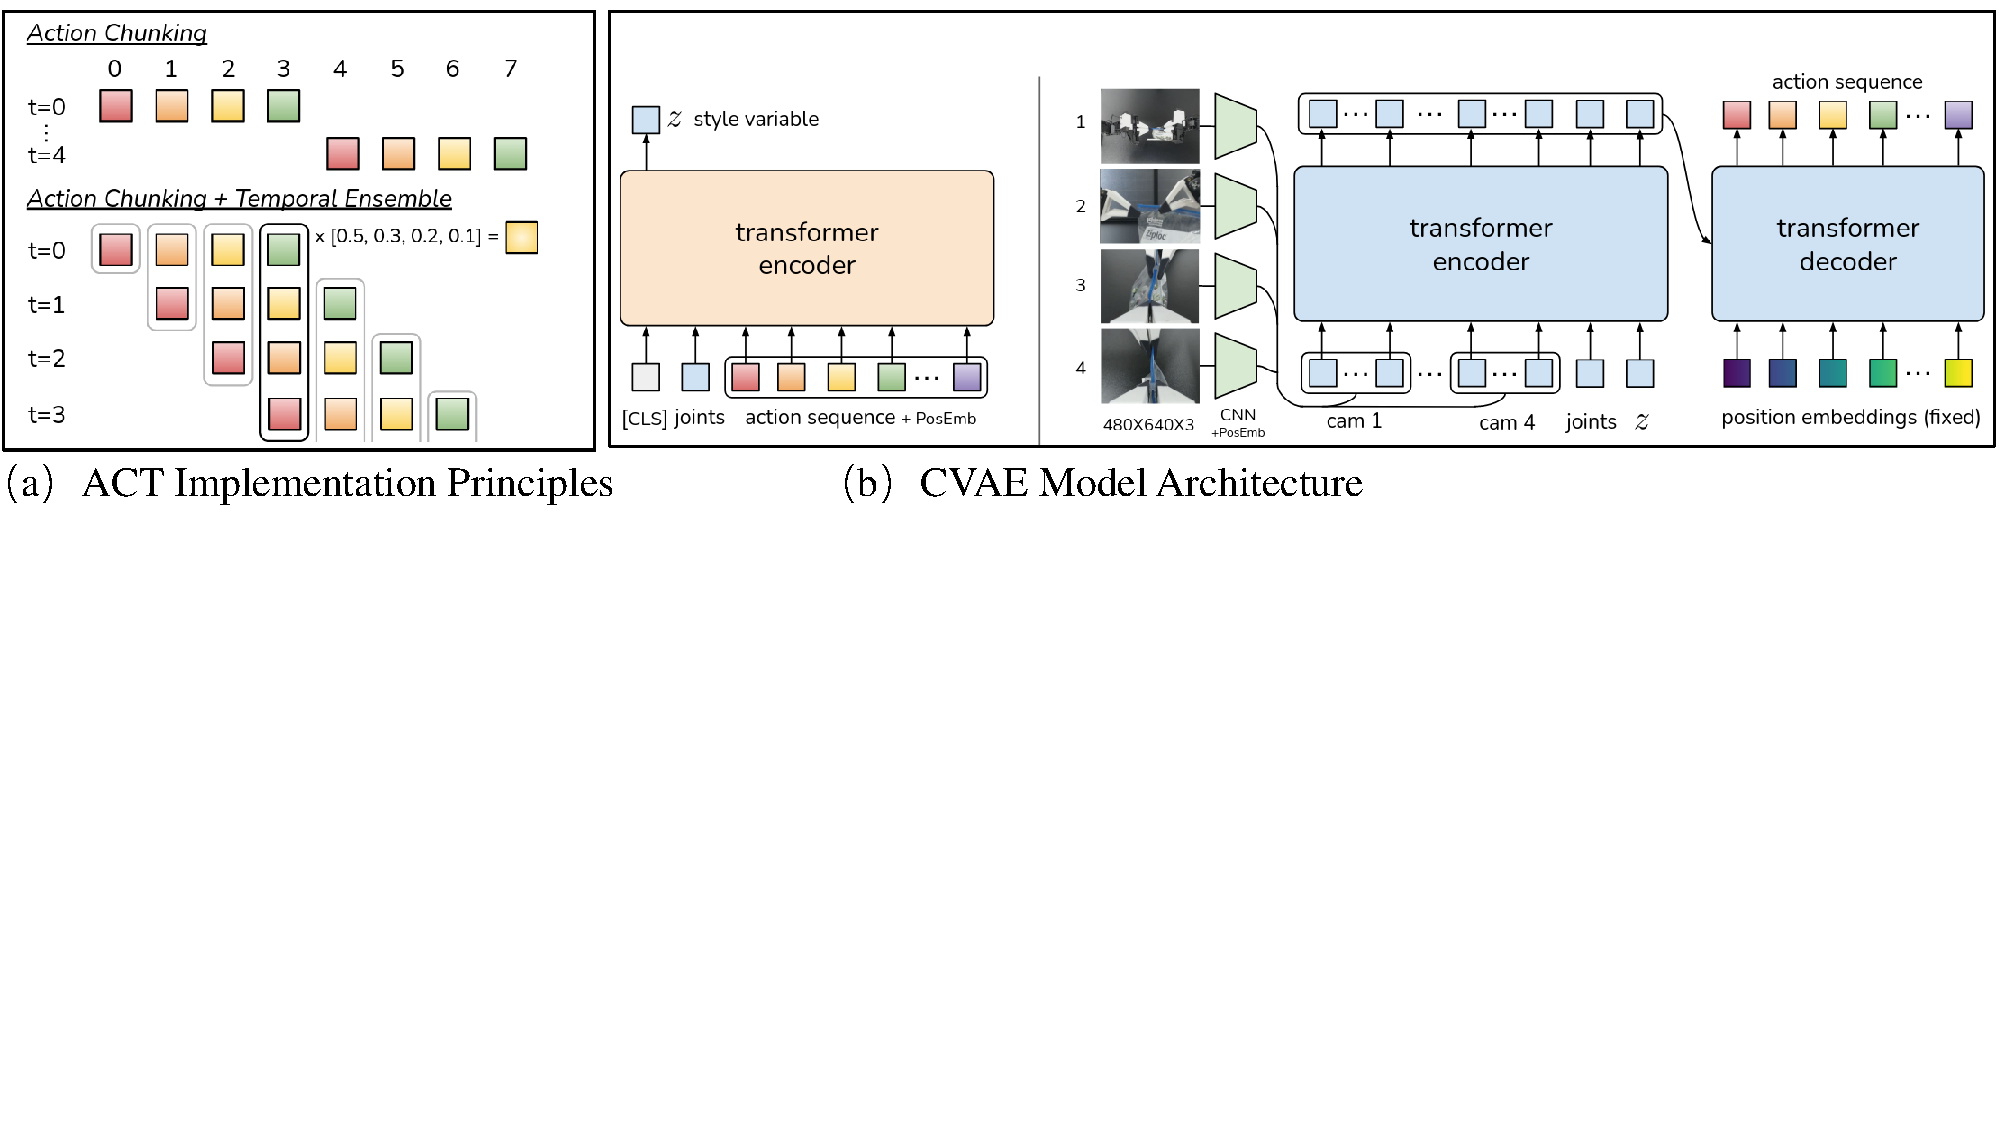
\includegraphics[width=\textwidth]{fig1.pdf}
\caption{ACT implementation principles and CVAE model architecture.}
\label{fig1}
\end{figure}



To better integrate the ACT algorithm into model training, the research team designed a Conditional Variational Autoencoder (CVAE) for policy training. This model takes the current observation as input, processes it through a ResNet, then encodes and decodes the features before outputting a sequence of predicted actions. The architecture of this model is illustrated in Fig.~\ref{fig1}(b) below.



\noindent The model's left side constitutes the CVAE encoder – containing a Transformer encoder, while the right side comprises the CVAE decoder – incorporating both a Transformer encoder and a Transformer decoder. During training, we primarily focus on the left-side operations: sampling RGB images and joint position tuples from human demonstration data to form corresponding action sequences as prediction targets (these action sequences are known predictions derived from the demonstration data), thereby obtaining the model's key parameter – the "style variable z".

The dimensional information of key components is presented in Table~\ref{tab:dim_summary} to clarify the model pipeline. The architecture follows a standard visual encoding and sequence modeling design: image features are first extracted and flattened, then fused with proprioceptive state and latent variables, and finally decoded into a sequence of predicted joint actions.


\begin{table}[htbp]
    \centering
	\caption{Dimensions of CVAE policy network modules}
	\label{tab:dim_summary}
	\begin{tabularx}{\textwidth}{@{}>{\hsize=0.5\hsize\centering\arraybackslash}X 
			>{\hsize=1.0\hsize\centering\arraybackslash}X 
			>{\hsize=0.8\hsize\centering\arraybackslash}X 
			>{\hsize=1.7\hsize\centering\arraybackslash}X@{}}
		\toprule
		\textbf{Module} & \textbf{Input Dim} & \textbf{Output Dim} & \textbf{Function} \\
		\midrule
		CNN & $4 \times 480 \times 640 \times 3$ & $1200 \times 512$ & Visual feature extraction \\
		Encoder & $1202 \times 512$ & $1202 \times 512$ & Fuse image, joints and latent $z$ \\
		Decoder & $k \times 512$ & $k \times 14$ & Generate $k$-step action sequence \\
		\bottomrule
	\end{tabularx}
\end{table}

\section{Experimental Setup and Methodology}
We primarily adopted the robotic arm structure from the huggingface/lerobot project on GitHub, which currently represents the most cost-effective solution capable of deploying this algorithm. To meet our requirements, we additionally procured cameras and other peripheral equipment. For different task scenarios, we designed corresponding experimental setups by adjusting grasping methods, camera positions, and training parameters to evaluate their respective success rates and task performance, thereby determining the optimal implementation approach and suitable application scenarios for this algorithm.

We selected two representative manipulation tasks: Tower of Hanoi, and dish washing. Here,Tower of Hanoi serves as a long-horizon task test, while dish washing represents daily task evaluation.

\subsection{Hardware Configuration}
Fig.~\ref{fig2-1} below illustrates the specific structure of our robotic arm system. The left side shows the follower arm responsible for object grasping, while the right side displays the leader arm used for manual operation to control the follower arm and record smooth demonstration datasets.


\begin{figure}
\centering
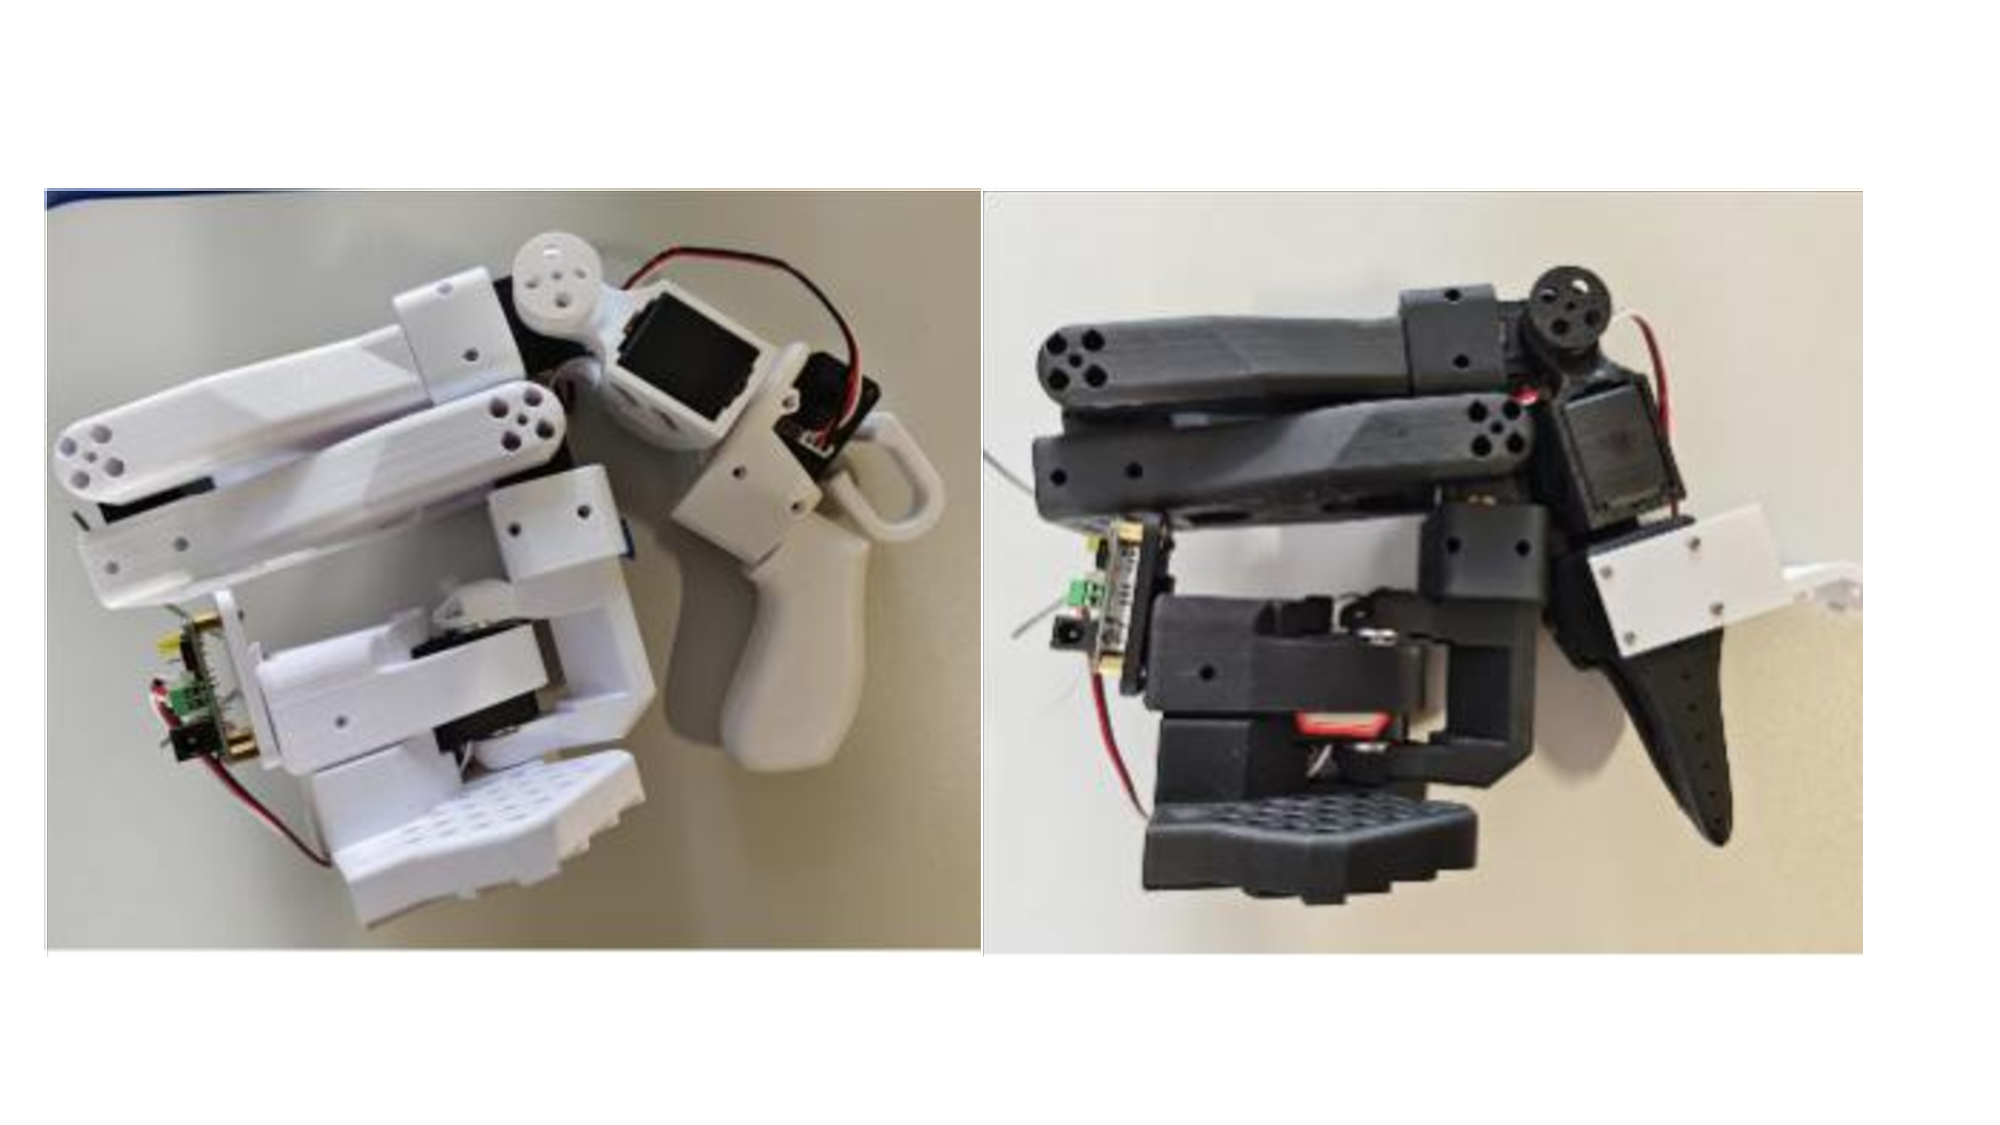
\includegraphics[width=\textwidth]{fig3.pdf}
\caption{Leader arm (Left) and follower arm(right).} \label{fig2-1}
\end{figure}

% \begin{figure}[htbp]
%   \centering
%   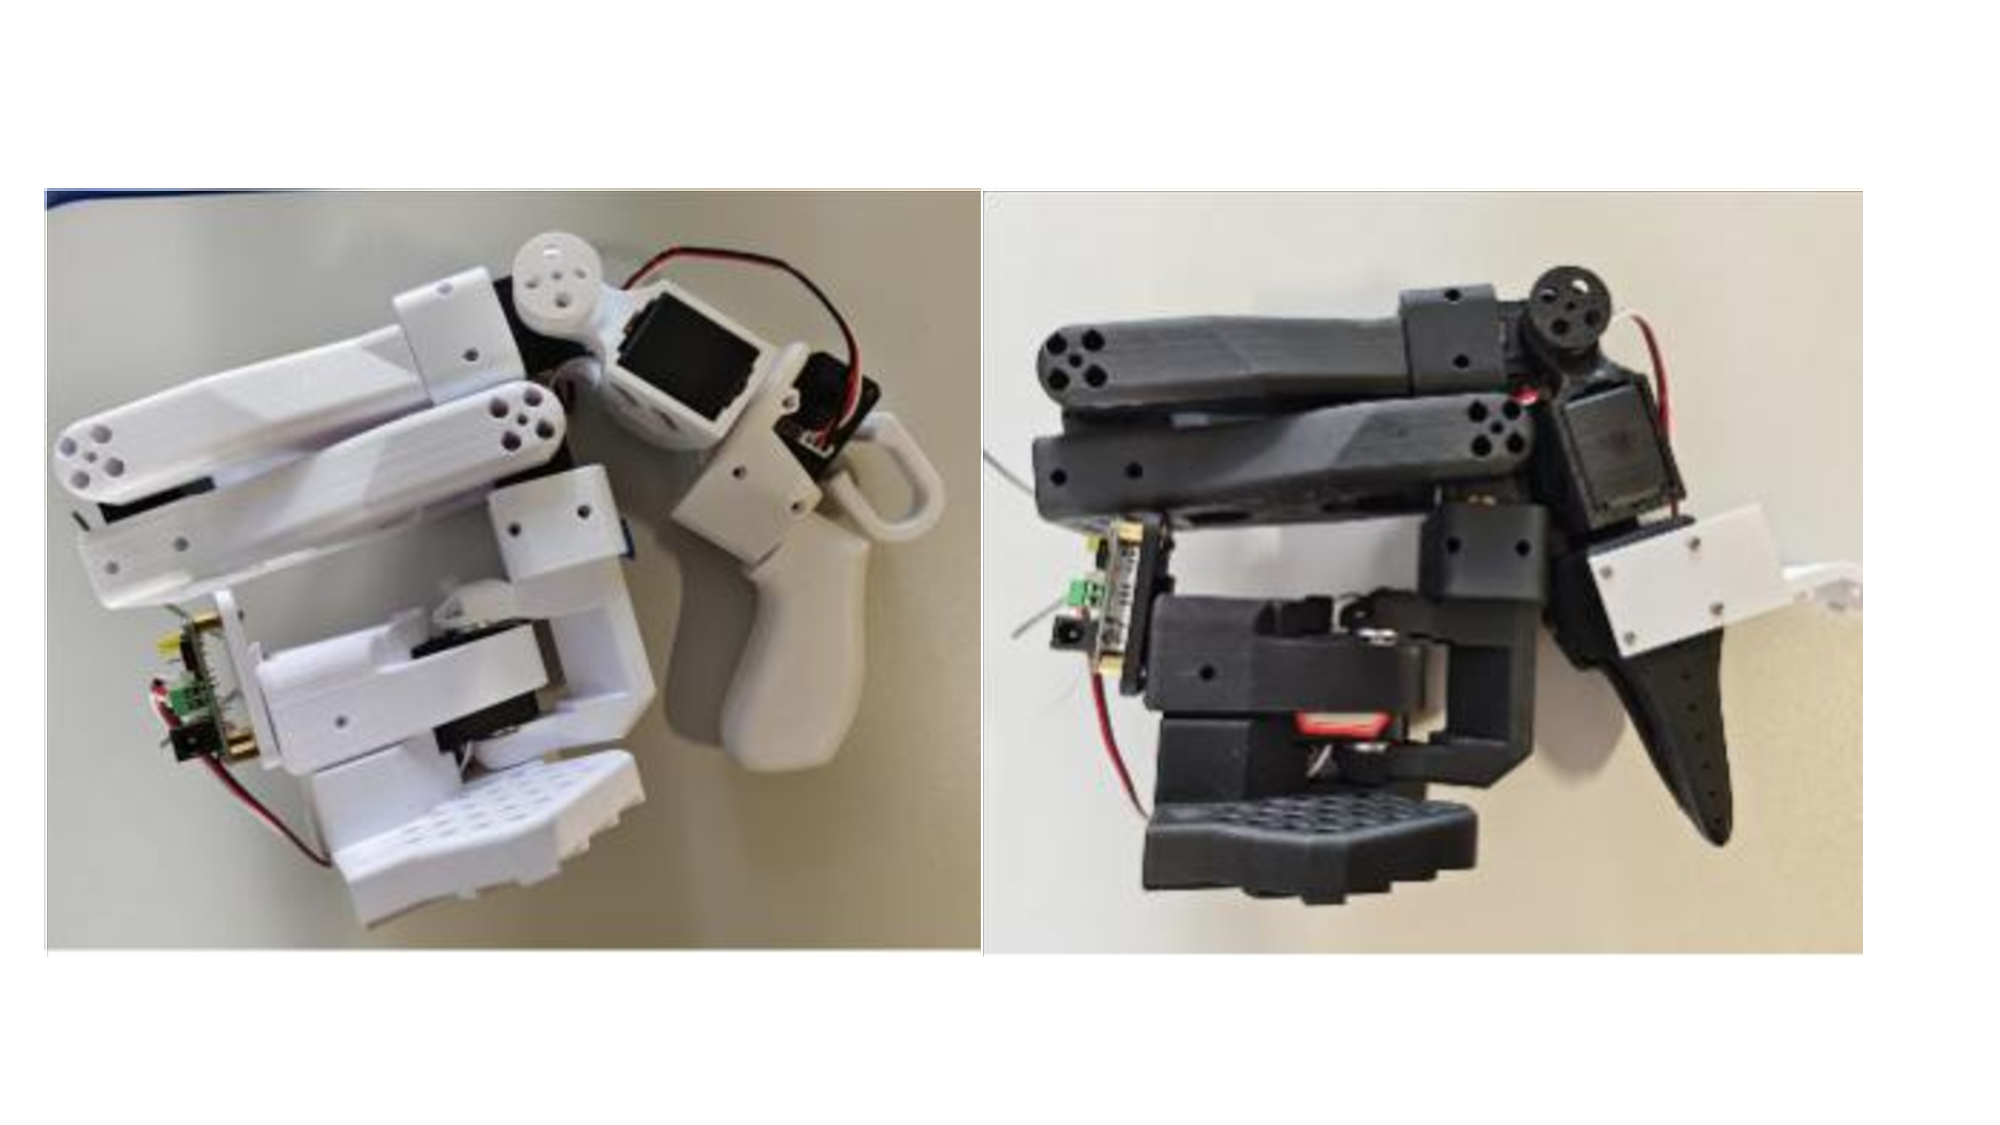
\includegraphics[height=3cm, width=\linewidth]{fig3.pdf} % 替换为你的图片路径
%   % \renewcommand{\arraystretch}{1.0} % 控制行间距(按需调整)
%   % \begin{tabular}{@{}m{0.3\textwidth}@{\hspace{0.05\textwidth}}m{0.3\textwidth}@{}}
%   %   \begin{minipage}{\linewidth}
%   %     \centering
%   %     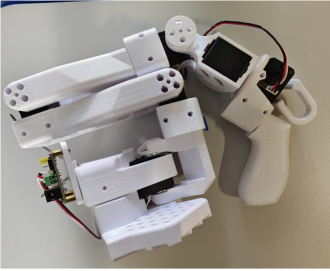
\includegraphics[height=3cm, width=\linewidth]{3.3} % 替换为你的图片路径
%   %   \end{minipage} &
%   %   \begin{minipage}{\linewidth}
%   %     \centering
%   %     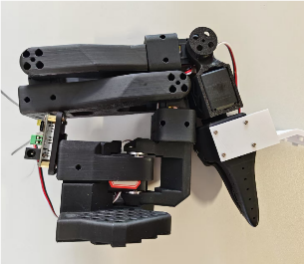
\includegraphics[height=3cm, width=\linewidth]{3.4} % 替换为你的图片路径
%   %   \end{minipage} \\
%   % \end{tabular}
%   % \caption{Main Title of the Figure} % 主标题
%   \label{fig:your_label} % 标签(用于引用)
% \end{figure}

\noindent Each 6-DOF robotic arm consists of a 3D-printed kit assembled with six 12V serial bus servos. For the leader arm, the transmission gears inside its servos were removed while retaining only the sensor functionality, thereby reducing servo resistance during data collection.


\begin{figure}
\centering
  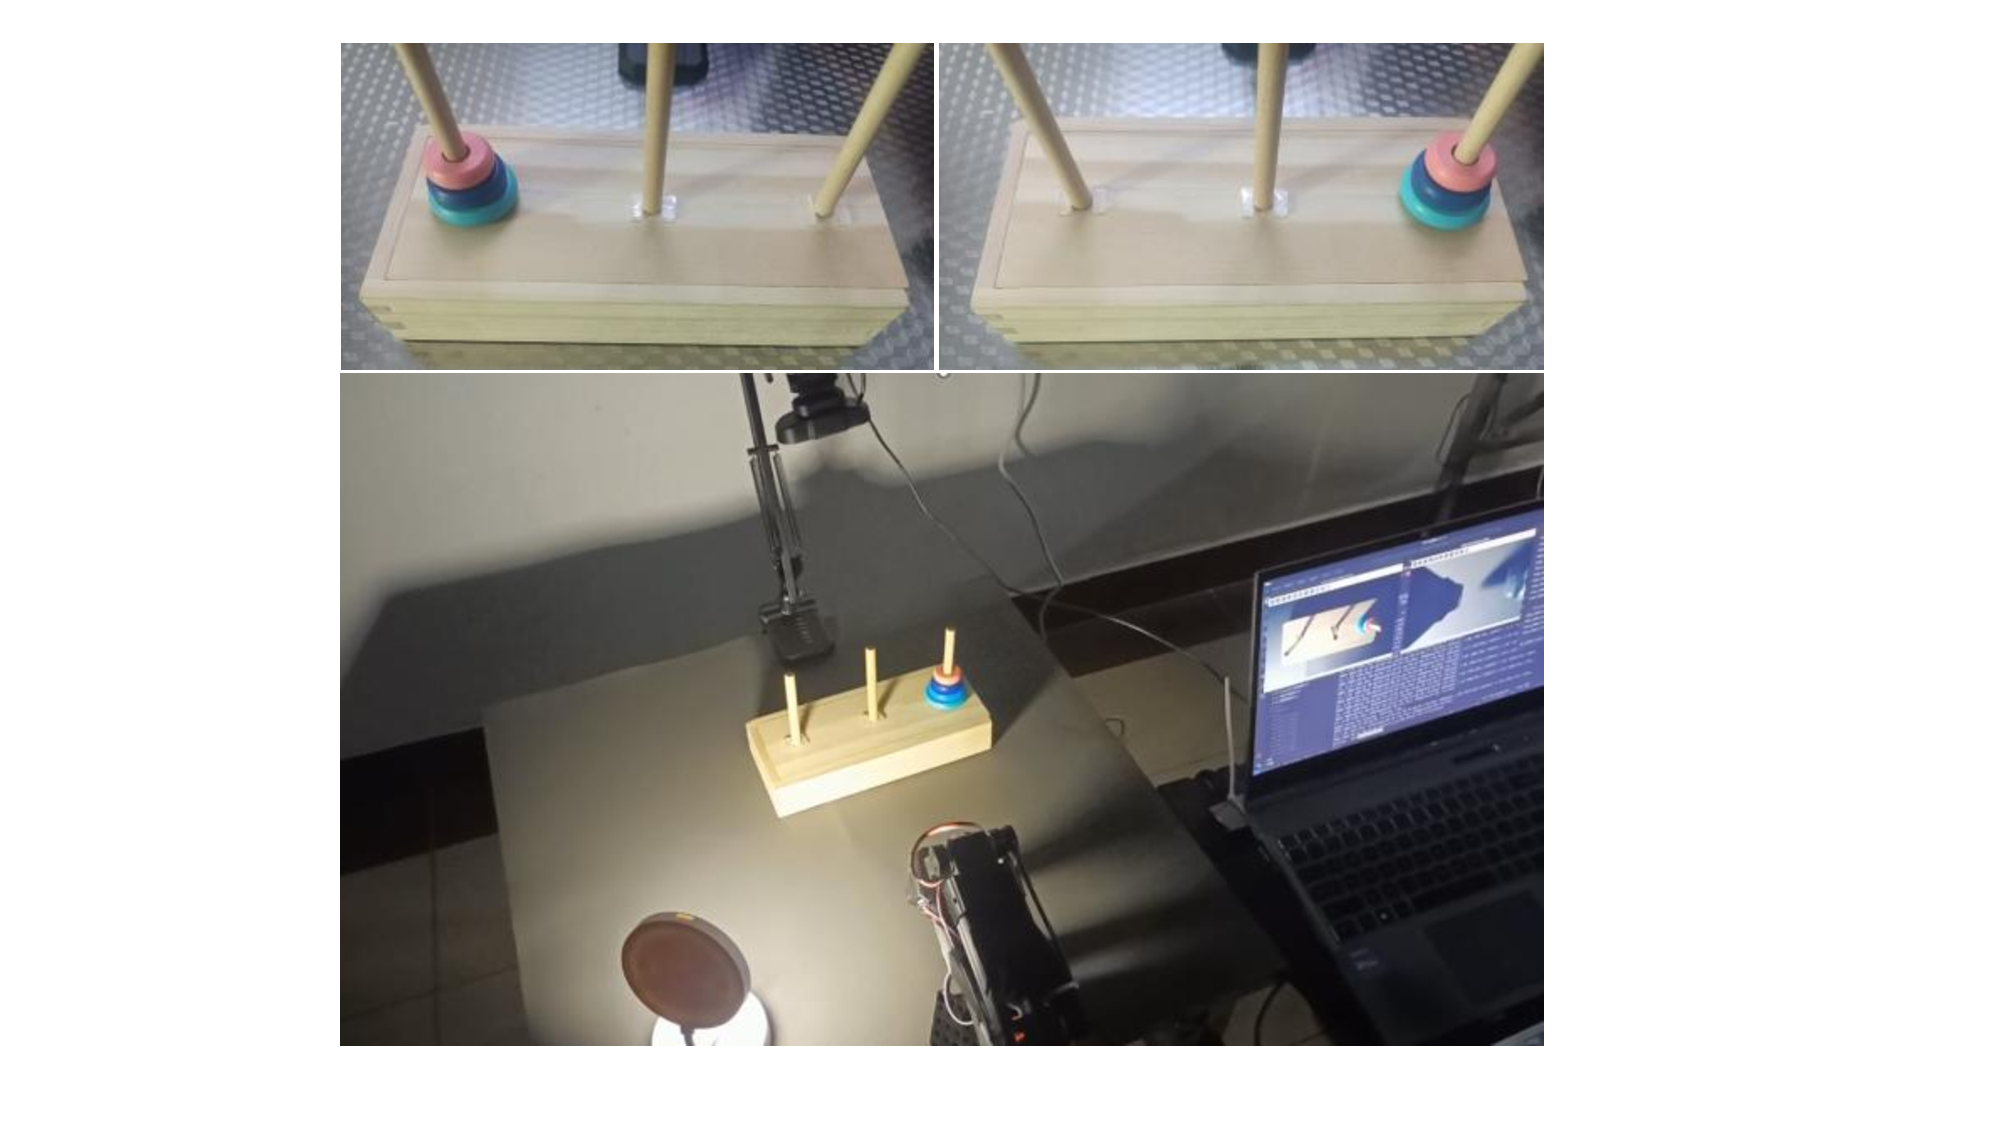
\includegraphics[width=0.95\textwidth]{fig4.pdf}
  \caption{ Initial state(upper left); target state(upper right);training environment(bottom).} \label{fig2}
  \end{figure}

\subsection{Tower of Hanoi task}

This task requires the robotic arm to autonomously relocate all four disks from the leftmost peg to the rightmost peg with minimal moves while strictly adhering to the Tower of Hanoi rules.

Fig.~\ref{fig2} displays the experimental setup for task implementation. We adopt the low-cost ViperX robotic arm architecture~\cite{ref1}~\cite{ref2}~\cite{ref3} to ensure system reproducibility.The hardware system draws inspiration from the modular design concept~\cite{ref4}, consisting of: an upper computer (laptop equipped with RTX 4060 discrete graphics card), lower computer (servo driver boards for master/slave robotic arms), and vision acquisition module (overhead global camera and wrist-mounted camera on the slave arm). In the experimental environment, the desk lamp, overhead camera, and Tower of Hanoi base remain fixed to eliminate interference from environmental variables on model accuracy.

Fig.~\ref{fig10} presents the complete workflow of this task. The process begins with the overhead global camera capturing the initial state image of the Tower of Hanoi setup. This visual data is then processed by the large language model ChatGPT-4o and adopts representation learning methods~\cite{ref5}, which performs image recognition to generate a corresponding digital state representation. The resulting digital representation serves as input parameters for the Tower of Hanoi solving algorithm, enabling the generation of an optimal sequence of movement actions. Finally, the control system executes these motion commands in sequence to autonomously complete the Tower of Hanoi solving task.

\begin{figure}[htbp]
\centering

\includegraphics[width=\textwidth]{10}
\caption{Overall workflow.}
 \label{fig10}
\end{figure}

\noindent This task optimized the positioning of the wrist-mounted vision system. As shown in Fig.~\ref{fig12}, the initial configuration (Position 1) exhibited tier recognition errors in multi-layered disc scenarios, primarily manifesting as erroneous grasps of second-layer discs with only a 40\% success rate. The wrist-mounted camera is crucial for precision operations~\cite{ref6}.By relocating the camera to the robotic gripper's center position (Position 2), precise tier recognition was achieved, significantly improving the grasping success rate to 90\%.

\begin{figure}[htbp]
\centering
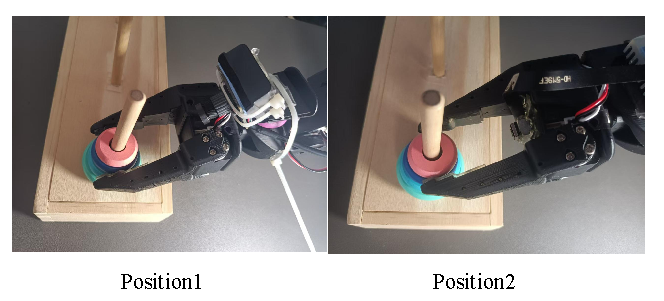
\includegraphics[width=0.85\textwidth]{fig12.pdf}
\caption{Wrist-mounted camera position adjustment.} \label{fig12}
\end{figure}



\noindent For the 4-layer Tower of Hanoi task, a total of 15 atomic disk-moving actions were identified, each requiring a separate model. Referencing hierarchical task decomposition methods~\cite{ref7}, 40 training episodes were initially collected per action, with each model trained for 100,000 steps. Due to potential teleoperation errors and lighting variations (e.g., between daytime and evening)\cite{ref8}, some models showed suboptimal validation performance. To enhance robustness, following design principles for home environments\cite{ref9}, additional data were collected and retraining was performed for underperforming models.

As shown in Fig.~\ref{fig14}, which illustrates the training loss curves for the first two models, all models achieved final training losses below 0.05, indicating stable convergence across the training process.


\begin{figure}
\centering
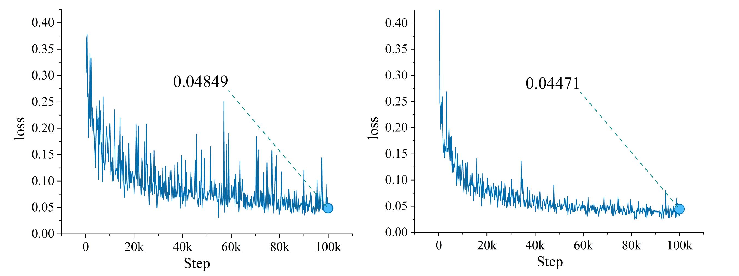
\includegraphics[width=323pt]{fig15.pdf}
\caption{The loss curve for the first two actions during model training.} \label{fig14}
\end{figure}


\noindent The validation success rates for models trained on the 15 decomposed actions are presented in Table~\ref{tab2}, with each model evaluated over 10 trials. 

\begin{table}
  \centering
    \caption{Model training specifications}\label{tab2}
  \begin{tabularx}{\textwidth}{
      >{\centering\arraybackslash}p{0.8cm}     % 第一列固定宽度(窄)
      >{\centering\arraybackslash}X           % 第二列自动调整
      >{\centering\arraybackslash}X  
      >{\centering\arraybackslash}X           % 第四列自动调整
      >{\centering\arraybackslash}X           % 第五列自动调整
      >{\centering\arraybackslash}X           % 第六列自动调整
    }
\toprule
    \textbf{step} & \textbf{action} & \textbf{state} & \textbf{training time} & \textbf{episodes} & \textbf{success rate} \\
   \midrule
     1 & A --> B      & A[1234]-B[]-C[]       & 2h 7m 51s  & 90 & 9/10 \\
     2 & A --> C      & A[123]-B[4]-C[]       & 2h 14m 43s & 40 & 9/10 \\
     3 & B --> C      & A[12]-B[4]-C[3]       & 2h 11m 19s & 50 & 10/10 \\
     4 & A --> B      & A[12]-B[]-C[34]       & 3h 46m 55s & 40 & 10/10 \\
     5 & C --> A      & A[1]-B[2]-C[34]       & 2h 7m 44s  & 80 & 10/10 \\
     6 & C --> B      & A[14]-B[2]-C[3]       & 2h 24m 28s & 40 & 9/10 \\
     7 & A --> B      & A[14]-B[23]-C[]       & 4h 13m 50s & 40 & 9/10 \\
     8 & A --> C      & A[1]-B[234]-C[]       & 3h 13m 1s  & 40 & 10/10 \\
     9 & B --> C      & A[]-B[234]-C[1]       & 1h 59m 21s & 70 & 10/10 \\
     10 & B --> A     & A[]-B[23]-C[14]       & 1h 58m 55s & 60 & 10/10 \\
     11 & C --> A     & A[3]-B[2]-C[14]       & 2h 5m 1s   & 50 & 10/10 \\
     12 & B --> C     & A[34]-B[2]-C[1]       & 3h 2m 31s  & 40 & 9/10 \\
     13 & A --> B     & A[34]-B[]-C[12]       & 2h 0m 38s  & 60 & 10/10 \\
     14 & A --> C     & A[3]-B[4]-C[12]       & 3h 28m 24s & 40 & 9/10 \\
     15 & B --> C     & A[]-B[4]-C[123]       & 2h 11m 32s & 70 & 10/10 \\
     \bottomrule
  \end{tabularx}
\end{table}


\noindent Action chunking mitigates error accumulation in long-horizon tasks by decomposing them into manageable units~\cite{ref10}. Experimental results demonstrate that while individual actions can achieve over 90\% success rate, the integrated task execution system's overall performance drops to 60\% (6/10) in sequential model deployment for the complete Tower of Hanoi task due to the bucket effect.

\subsection{Dual-Arm Cooperative Tableware Cleaning Task}
Based on bimanual coordination theory~\cite{ref11}, this task employs a dual master-slave arm configuration to achieve human-like bimanual manipulation for plate wiping. This task employs a dual master-slave arm system with a three-camera setup, selecting a dish-cleaning scenario in a household context to simulate bimanual operation. Fig.~\ref{fig9} illustrates the task environment configuration. The setup consists of a pair of blue master-slave arms and a pair of white master-slave arms. The two master arms are responsible for teleoperating the slave arms to collect data, while the other two master arms execute the final dish-cleaning task. The triple-camera system is adopted, analogous to visual policy optimization~\cite{ref12}, leveraging multi-camera fusion strategies~\cite{ref13} by combining global, frontal, and side-view cameras for full-process monitoring. Multi-perspective fusion of global and wrist cameras enhances precision: a global camera fixed overhead records the workspace to guide plate-wiping; a front-facing camera mounted centrally directs the blue arm to grasp the plate edge; a downward-facing camera on the left ensures precise placement at the target location (marked with a red tag). On the table, a soiled plate is placed in the center, with a sponge placed on the right side. A desk lamp is installed near the bracket to provide supplemental lighting, ensuring consistent illumination for the experiment.

\begin{figure}
\centering
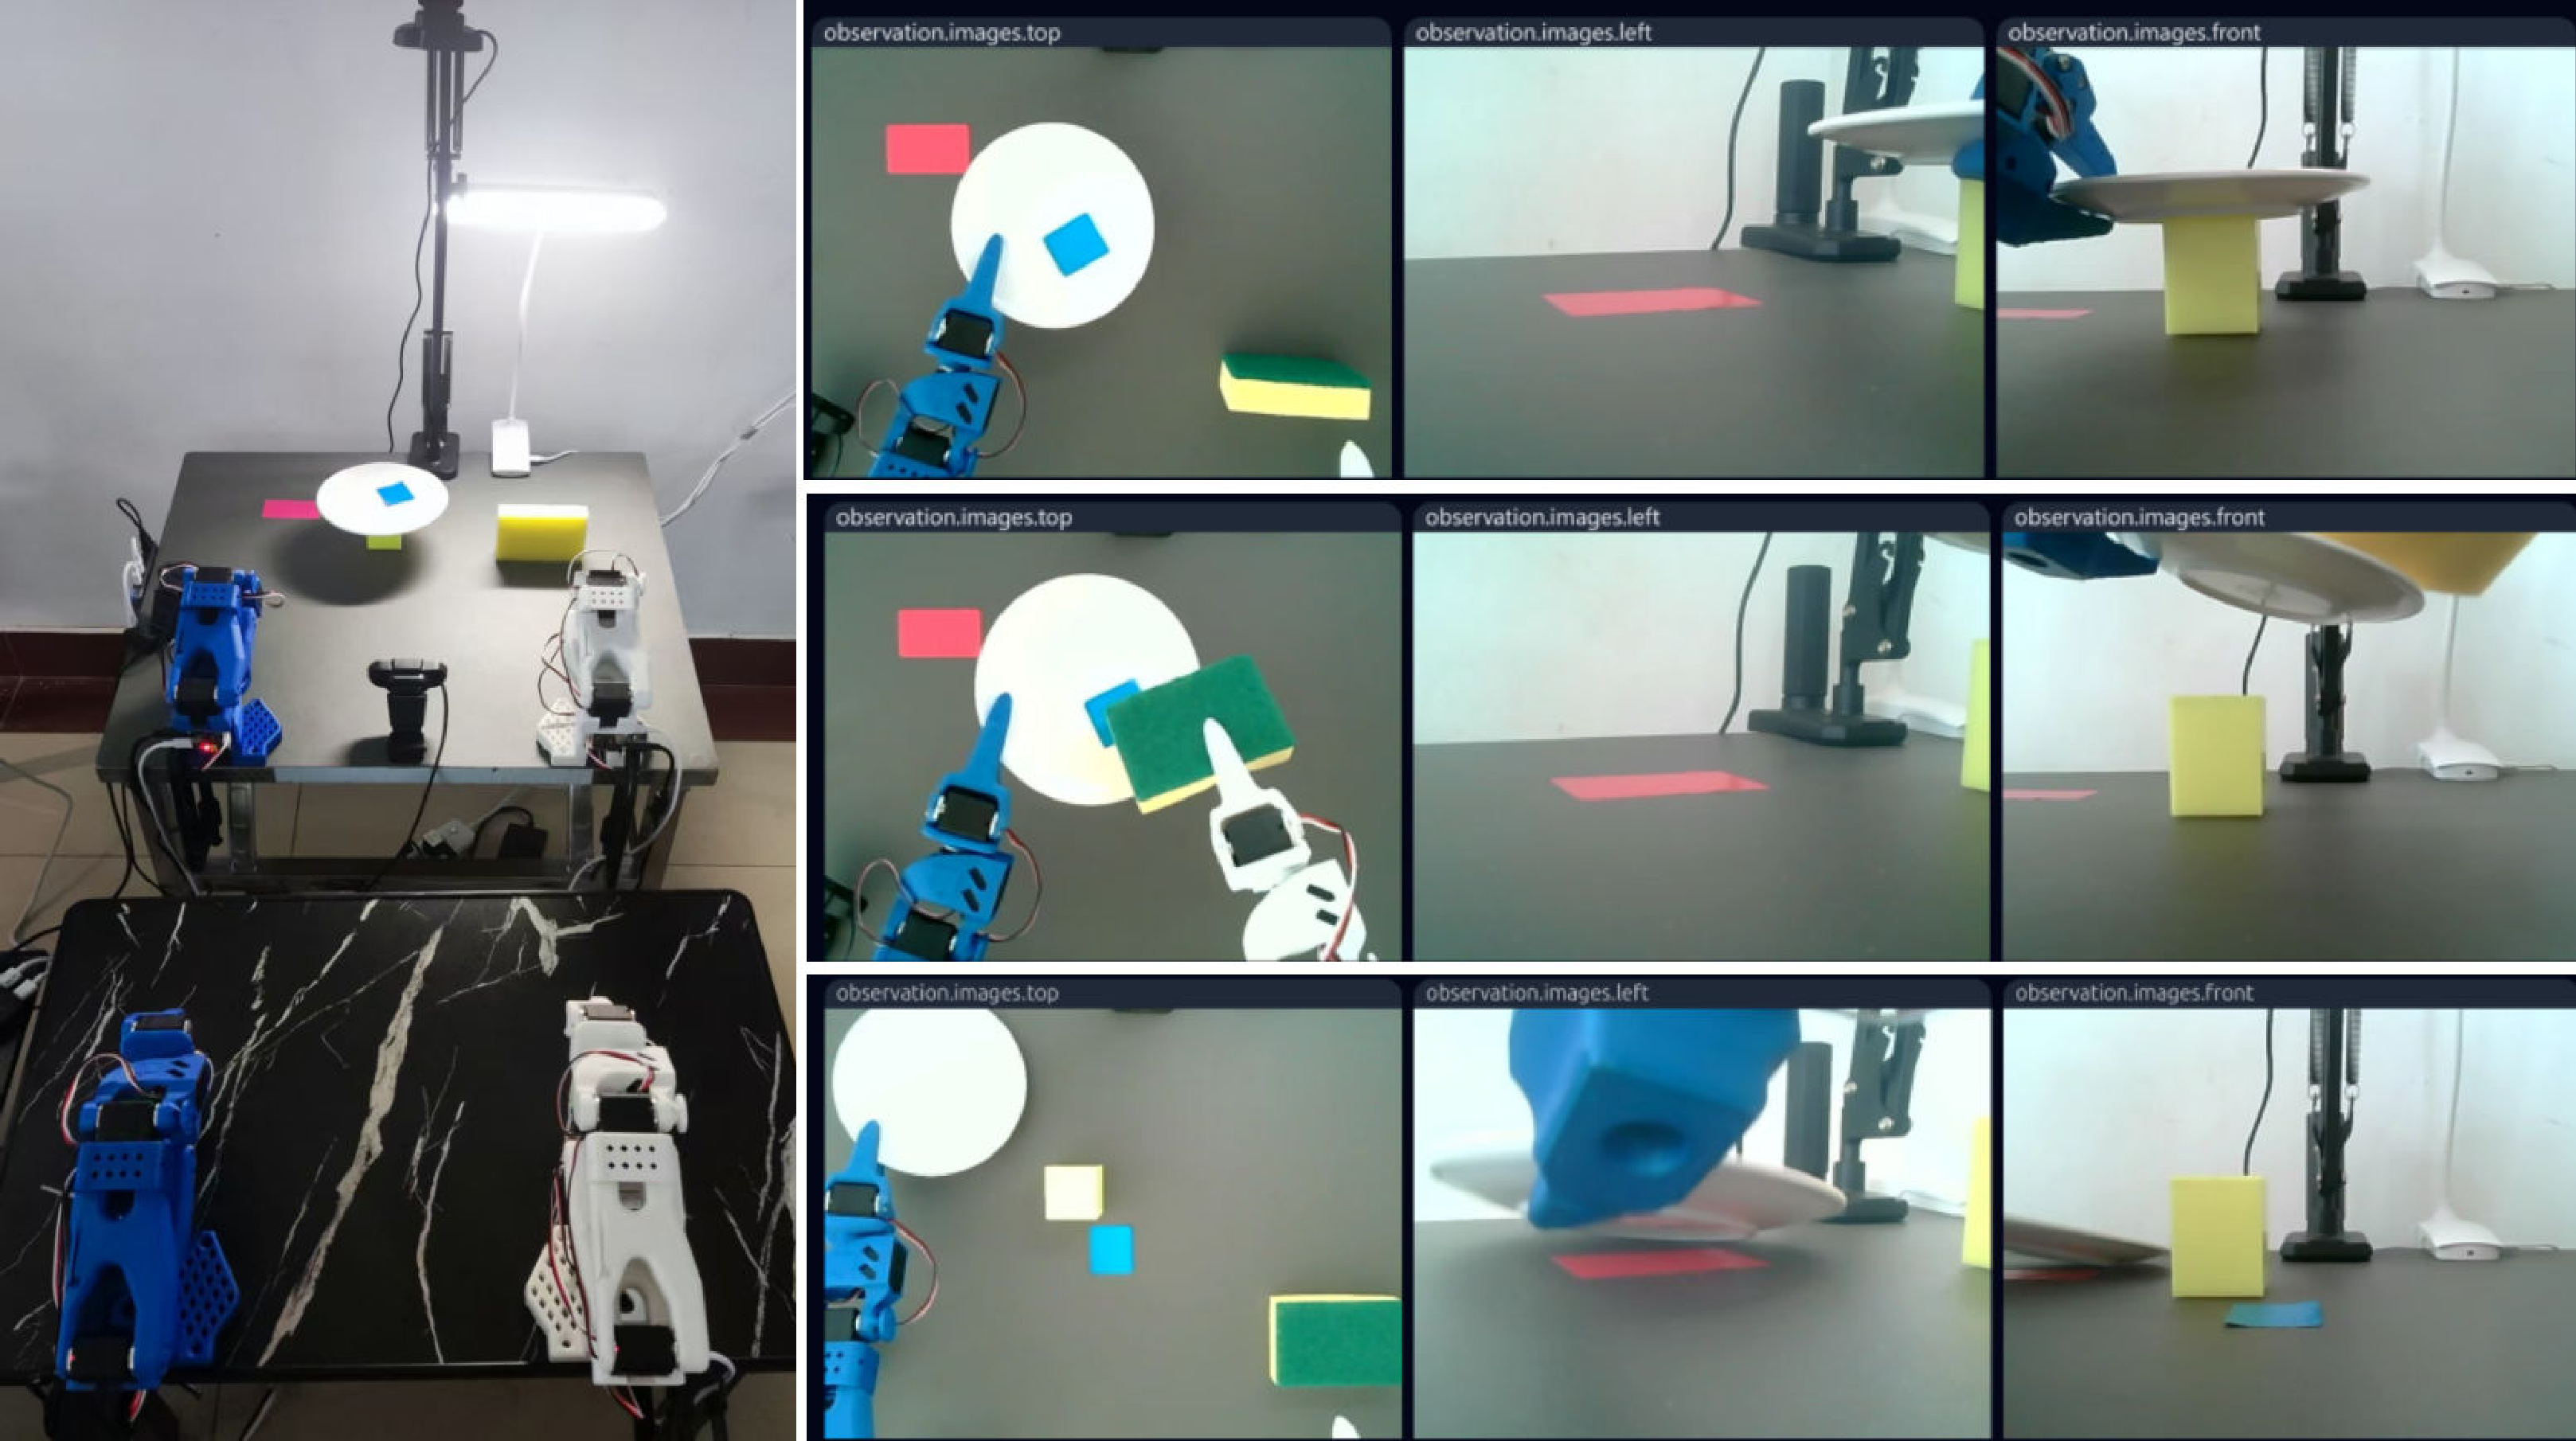
\includegraphics[width=\textwidth]{fig9.pdf}
\caption{ Training environment and task workflow} \label{fig9}
\end{figure}


Fig.~\ref{fig9} illustrates the entire task workflow. It begins with the global-view camera identifying the soiled plate. The blue robotic arm then moves to the plate's position and, guided by the mid-level camera, precisely grips the plate's edge. Next, the white robotic arm picks up the sponge and wipes the stains off the plate until the global-view camera confirms the plate is clean~\cite{fu_deep_2022}. The white arm then releases the sponge and returns to its initial position. Subsequently, the blue robotic arm, guided by the side-view camera, accurately places the cleaned plate onto the designated spot (marked with a red positioning tag) before resetting. This concludes the task.


The conventional LeRobot framework was only suitable for single-arm static task scenarios. To enable bimanual operation emulation, this study extensively customized the LeRobot framework with reference to Transformer architecture extension methods . The enhanced framework now supports dual robotic arms, multiple cameras, and 7-DOF robotic arms, capable of automatically determining camera and robotic arm status parameters during data collection and training while adhering to human-robot interaction guidelines~\cite{ref15}. This achieves a fully customizable pipeline encompassing teleoperation data collection, model training, and model deployment.


As demonstrated by the Open X-Embodiment team~\cite{ref16}, cross-task collaborative training can enhance data efficiency. For this task, we collected 30 episodes of teleoperation data for the dual-arm dish-cleaning task and conducted model training on a platform equipped with an RTX 4090 GPU. The relevant training parameters and data are presented in Fig.~\ref{fig19} below.


\begin{figure}
\centering
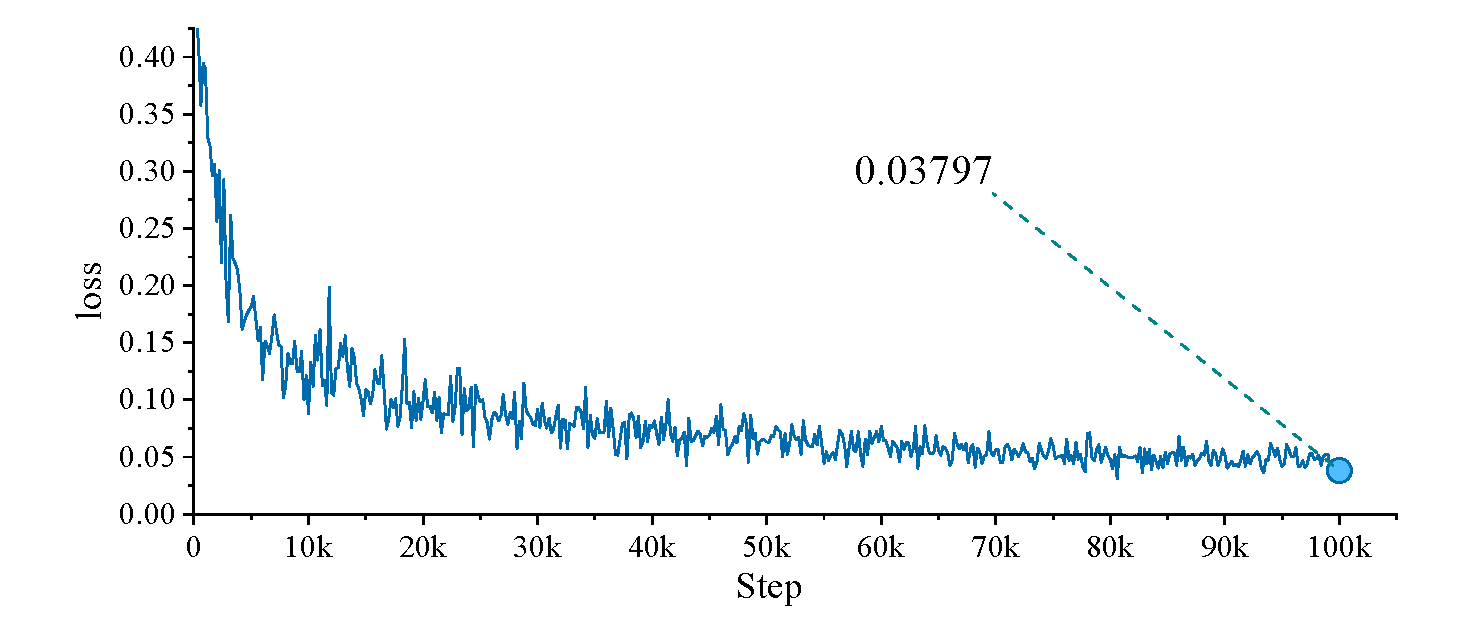
\includegraphics[width=323pt]{fig8.pdf}
\caption{Loss curve.} \label{fig19}
\end{figure}


\noindent After completing model training, we deployed it to the host computer for validation. The test results demonstrate that whenever the global-view camera detects a soiled plate, the dual robotic arms automatically execute the dish-cleaning operation. This process repeats until all stains are removed, after which the cleaned plate is precisely placed at the designated location. Experimental validation confirmed the model achieves an accuracy of 70\%, proving its effectiveness in completing the task.

These findings suggest that for similar daily-life tasks, the proposed solution only requires minimal additional data collection and training to deliver comparable performance. This approach shows strong potential for implementation in future intelligent robotic systems.As demonstrated by Shafiullah\cite{ref17}, this approach can be generalized to other household tasks, adapting to new scenarios with minimal data.


\section{Conclusion}
The two experiments above demonstrate that the ACT algorithm can reduce costs while meeting practical task requirements, making it suitable for real-world applications like factory robotic arms and household service robots. Although still constrained by hardware limitations and the scale/quality of demonstration datasets - preventing true task generalization - its end-to-end learning approach significantly decreases deployment costs and implementation barriers, enabling rapid adaptation to diverse complex daily tasks.

\subsubsection{Acknowledgments} This research was supported by the National College Student Innovation and Entrepreneurship Training Program of China under project numbers 202410559078 and 202310559124.


% \begin{REF}
  % \vspace{-50pt}
  % \bibliography{ref}%参考文献
  % \end{REF}
% \begin{thebibliography}{8}
% \bibitem{ref1} 
% ViperX 300 S [EB/OL]. [2025-03-31]. \url{https://www.trossenrobotics.com/viperx-300}

% \bibitem{ref2} 
% WidowX 250 S [EB/OL]. [2025-03-31]. \url{https://www.trossenrobotics.com/widowx-250}

% \bibitem{ref3} 
% RE2, INC. Highly Dexterous Manipulation System - Capabilities - Part 1 [Z/OL]. (2014-11-08)[2025-03-31]. \url{https://www.youtube.com/watch?v=TearcKVj0iY}

% \bibitem{ref4} 
% Wyborek K A, Berger E H, Van Der Loos H F M, et al. Towards a personal robotics development platform: Rationale and design of an intrinsically safe personal robot [C]//2008 IEEE International Conference on Robotics and Automation. 2008: 2165-2170

% \bibitem{ref5} 
% Pari J, Shafiullah N M, Arunachalam S P, et al. The Surprising Effectiveness of Representation Learning for Visual Imitation [J]. arXiv, 2021.

% \bibitem{ref6} 
% Hsu K, Kim M J, Rafailov R, et al. Vision-Based Manipulators Need to Also See from Their Hands [J]. arXiv, 2022. 

% \bibitem{ref7} 
% Kroemer O, Daniel C, Neumann G, et al. Towards learning hierarchical skills for multi-phase manipulation tasks [C]//2015 IEEE International Conference on Robotics and Automation (ICRA). Seattle, WA, USA: IEEE, 2015: 1503-1510

% \bibitem{ref8} 
% Shi L X, Sharma A, Zhao T Z, et al. Waypoint-Based Imitation Learning for Robotic Manipulation [J]. arXiv, 2023. 

% \bibitem{ref9} 
% Gupta A, Murali A, Gandhi D, et al. Robot Learning in Homes: Improving Generalization and Reducing Dataset Bias [J]. arXiv, 2018. \url{http://arxiv.org/abs/1807.07049}. DOI:10.48550/arXiv.1807.07049

% \bibitem{ref10} 
% Shafiullah N M M, Cui Z J, Altanzaya A, et al. Behavior Transformers: Cloning \$k\$ modes with one stone [J]. arXiv, 2022. 

% \bibitem{ref11} 
% Smith C, Karayiannidis Y, Nalpantidis L, et al. Dual arm manipulation—A survey [J]. Robotics and Autonomous Systems, 2012, 60(10): 1340-1353

% \bibitem{ref12} 
% Chi C, Xu Z, Feng S, et al. Diffusion Policy: Visuomotor Policy Learning via Action Diffusion [J]. arXiv, 2024. 

% \bibitem{ref13} 
% Brohan A, Brown N, Carbajal J, et al. RT-1: Robotics Transformer for Real-World Control at Scale [J]. arXiv, 2023. 

% \bibitem{ref14} 
% Fu Z, Cheng X, Pathak D. Deep Whole-Body Control: Learning a Unified Policy for Manipulation and Locomotion [J]. arXiv, 2022. 

% \bibitem{ref15} 
% Dragan A D, Lee K C T, Srinivasa S S. Legibility and predictability of robot motion [C]//2013 8th ACM/IEEE International Conference on Human-Robot Interaction (HRI). Tokyo, Japan: IEEE, 2013: 301-308

% \bibitem{ref16} 
% Collaboration O X E, O'Neill A, Rehman A, et al. Open X-Embodiment: Robotic Learning Datasets and RT-X Models [J]. arXiv, 2024. 

% \bibitem{ref17} 
% Shafiullah N M M, Rai A, Etukuru H, et al. On Bringing Robots Home [J]. arXiv, 2023. 
% \end{thebibliography}





%
% the environments 'definition', 'lemma', 'proposition', 'corollary',
% 'remark', and 'example' are defined in the LLNCS documentclass as well.
%


%
% ---- Bibliography ----
%
% BibTeX users should specify bibliography style 'splncs04'.
% References will then be sorted and formatted in the correct style.
%
\bibliographystyle{splncs04}
\bibliography{ref}
%
\end{document}
